\documentclass[9pt]{beamer}
\mode<presentation>
\usepackage[T1]{fontenc}
\usepackage{color}
\usepackage{graphicx}
\usepackage{natbib}
\usepackage{tikz}
\usetikzlibrary{shapes.geometric}
\usepackage{xmpmulti}
\usepackage{animate}
\usepackage{tcolorbox}
\usepackage{amsmath}
\usepackage{gensymb}
\usepackage{csquotes}
\usepackage{bibentry}
\nobibliography*

\usetheme{Singapore}

\setbeamercolor{block title}{bg=structure!20}
\setbeamercolor{block body}{bg=structure!10}
\setbeamertemplate{blocks}[rounded][shadow]
%\usecolortheme{seahorse}

\usefonttheme{professionalfonts}

\title[Climate Impacts]{Scaling up assessments of regional impacts of climate change: a rapid, computer-assisted systematic map}
\author{Max Callaghan, Jan Minx, Carl-Friedrich Schleussner, Gerrit Hansen, Quentin Lejeune, Shruti Nath, Emily Theokritoff, Marina Andrijevic, Robert Brecha, Michael Hegarty, Chelsea Jones, Kaylin Lee, Agathe Lucas, Nicole van Maanen, Inga Menke, Peter Pfleiderer, Burcu Yesil }
\institute[MCC]{
	\includegraphics[height=1cm,width=2cm]{images/MCC_Logo_RZ_rgb.jpg} \hspace{5em} \includegraphics[height=1cm]{images/climate_analytics.png}
}

\newif\ifframeinlbf
\frameinlbftrue
\makeatletter
\newcommand\listofframes{\@starttoc{lbf}}
\makeatother

\addtobeamertemplate{frametitle}{}{%
	\ifframeinlbf
	\addcontentsline{lbf}{section}{\protect\makebox[2em][l]{%
			\protect\usebeamercolor[fg]{structure}\insertframenumber\hfill}%
		\insertframetitle\par}%
	\else\fi
}

\newtheorem*{remark}{}

\bibliographystyle{apalike}

\begin{document}
	
\begin{frame}
	\titlepage
\end{frame}


%%%%%%%%%%%%%%%%%%%%%%%%%%%%%%%%%%%%%%%%%%%%%%%%%%
%% Introduction
\section{Introduction}

\begin{frame}
\tableofcontents[currentsection]
\end{frame}

\begin{frame}{Context}

Systematic assessments of the evidence on Climate Change like those conducted by the IPCC are vital.

\begin{columns}
	\begin{column}{0.618\linewidth}
		\begin{figure}
			\includegraphics[width=\linewidth]{../map_18.png}<1->
		\end{figure}
	\end{column}
	\begin{column}{0.312\linewidth}
		
		\begin{figure}
			\includegraphics[width=\linewidth]{images/pubs_time_wgb_lp.pdf}<2->
		\end{figure}
		
		\begin{itemize}
			\small
			\item<2->These are challenged by big literature \cite{Callaghan2020} 
			\item<3->They do not account for uncertainty about what literature is available
		\end{itemize}
	\end{column}
\end{columns}

\end{frame}

\begin{frame}{Quantifying the literature}

\begin{columns}
	
	\begin{column}{0.382\linewidth}
	\begin{itemize}
		\item AR5 WGII started with a basic bibliometric analysis of climate change (and impacts and adaptation) literature
		\item The literature has doubled again since then
		\item We can do more than this
	\end{itemize}
\end{column}

	\begin{column}{0.618\linewidth}
		\begin{figure}
			\includegraphics[width=0.7\textheight]{ar5_fig_1_1}
		\end{figure}
	\end{column}

\end{columns}

\end{frame}


\begin{frame}{Goal}
There are hundreds of thousands of documents potentially relevant to observed climate impacts. We want to be able to do two things:

\begin{itemize}
	\item<2-> Separate those documents which \textit{are} relevant from those that are not
	\item<3-> Predict in what way relevant documents are relevant:
	\begin{itemize}
		\item What impacts do they document?
		\item What type of evidence do they provide?
		\item In which locations is there evidence
	\end{itemize}
\end{itemize}

\only<4->{Once we can do that, we can draw a rough map of the available evidence, and aid the production of an \textit{assessment} of the available evidence}

\end{frame}



\begin{frame}{Distribution of labour between humans and machines - the ``Dangerous Supplement''}

A human expert or a team of human experts is best placed to answer those questions for any single document, but they can't look at all potentially relevant documents

\bigskip

We can use labels generated by humans to try to teach a computer what a relevant document looks like, and how to decide in what way it is relevant. 

\bigskip

If this works well, we can predict, with some uncertainty, how much evidence there is, and where and on what topic it is.

\end{frame}


%%%%%%%%%%%%%%%%%%%%%%%%%%%%%%%%%%%%%%%%%%%%%%%%%%
%% Data
\section{Data collection}

\begin{frame}
\tableofcontents[currentsection]
\end{frame}

\begin{frame}{Building a query}

We built a query using the documents from the tables in AR5 WGII Chapter 18.

The ideal query should contain \textit{all} documents included in those tables, along with \textit{all} additional relevant documents (untestable) and a hopefully minimal amount of irrelevant documents

\begin{figure}
	\includegraphics[width=0.7\linewidth]{../plots/basic_lit_plot.png}<1>
	\includegraphics[width=0.7\linewidth]{../plots/lit_plot_query_1.png}<2>
	\includegraphics[width=0.7\linewidth]{../plots/lit_plot_query_3.png}<3>
	\includegraphics[width=0.7\linewidth]{../plots/lit_plot_query_2.png}<4>
\end{figure}
\end{frame}

\begin{frame}{Our query contained a list of climate variables, a list of impacts, and a list of words narrowing down the literature on observed impacts}

\begin{columns}
	\begin{column}{0.33\linewidth}
		\textbf{Climate}
		
		\scriptsize
		
		TS=("climate model" OR "elevated* temperatur" OR "ocean* warming" OR "saline* intrusion" OR "chang* climat" OR "environment* change" OR "climat* change" OR "climat* warm" OR "warming* climat" OR "climat* varia" OR "global* warming" OR "global* change" OR "greenhouse* effect" OR "snow cover" OR "extreme temperature" OR "cyclone" OR "ocean acidification" OR "anthropogen*" OR "sea* level" OR "precipitation variabil*" OR "precipitation change*" OR "temperature* impact" OR "environmental* variab" OR "weather* pattern" OR "weather* factor*" OR "climat*") OR TS=("change* NEAR/5 cryosphere" OR "increase* NEAR/3 temperatur*")) 
		
	\end{column}
	\begin{column}{0.33\linewidth}
		
		\textbf{Impacts}
		
		\scriptsize
		
		AND (TS=("migration" OR "impact*" OR "specie*" OR "mortality*" OR "health" OR "disease*" OR "ecosystem*" OR "mass balance" OR "flood*" OR "drought" OR "disease*" OR "adaptation" OR "malaria" OR "fire" OR "water scarcity" OR "water supply" OR "permafrost" OR "biological response" OR "food availability" OR "food security" OR "vegetation dynamic*" OR "cyclone*" OR "yield*" OR "gender" OR "indigenous" OR "conflict" OR "inequality" OR "snow water equival*" OR "surface temp*") OR TS=("glacier* NEAR/3 melt*" OR "glacier* NEAR/3 mass*" OR "erosion* NEAR/5 coast*" OR "glacier* NEAR/5 retreat*" OR "rainfall* NEAR/5 reduc*" OR "coral* NEAR/5 stress*" OR "precip* NEAR/5 *crease*" OR "river NEAR/5 flow"))
		
	\end{column}
	\begin{column}{0.33\linewidth}
		
		\textbf{Observed}
		
		\scriptsize
		
		AND (TS=("recent" OR "current" OR "modern" OR "observ*" OR "evidence*" OR "past" OR "local" OR "region*" OR "significant" OR "driver*" OR "driving” OR "respon*" OR "were responsible" OR "was responsible" OR "exhibited" OR "witnessed" OR "attribut*" OR "has increased" OR "has decreased" OR "histor*" OR "correlation" OR "evaluation") )
	\end{column}	
\end{columns}

\end{frame}

\begin{frame}{We set up our platform to record the relevance and lots of other information about each document}

\begin{figure}
	\includegraphics[width=\linewidth]{../plots/screening-platform}
\end{figure}

\end{frame}

\begin{frame}{Screening and coding}

\begin{columns}
	\begin{column}{0.382\linewidth}
		\begin{itemize}
			\item 1 large random sample (unbalanced)
			\item 1 sample of documents predicted to be relevant (unbalanced)
			\item iterative small samples of documents predicted to be relevant to each category (over-hasty generalisation)
			\item iterative samples of documents containing words and phrases designed to pick up under-represented (subject to human bias and error)
		\end{itemize}
	\end{column}
	\begin{column}{0.618\linewidth}
		\begin{figure}
			\includegraphics[width=\linewidth]{../plots/progress/docs_time.pdf}
		\end{figure}
	
	\medskip 
	
	To which we added the papers included in AR5 WGII Chapter 18 (coded as relevant and with their corresponding impact category).
	\end{column}
\end{columns}



\end{frame}



%%%%%%%%%%%%%%%%%%%%%%%%%%%%%%%%%%%%%%%%%%%%%%%%%%
%% Machine learning
\section{Machine learning}

\begin{frame}
\tableofcontents[currentsection]
\end{frame}

\begin{frame}{Feature space - text as data}

The set of features is a TFIDF weighted set of unigrams and bigrams from the documents' abstracts

\medskip

\begin{columns}
	\begin{column}{0.5\linewidth}
		\includegraphics[width=\linewidth]{images/doc_example.png}
	\end{column}
	\begin{column}{0.5\linewidth}
		\includegraphics[width=\linewidth]{images/example_doc_tfidf.pdf}
	\end{column}
\end{columns}

\medskip

We discard very uncommon and very common features, leaving us with a vocabulary of 7,394 unique features.

\end{frame}

\begin{frame}{Setup}
We need two types of classifiers:
\begin{itemize}
	\item A binary, include/don't include classifier
	\item Various multilabel classifiers for impact types, attribution categories and climate drivers
\end{itemize}

\begin{columns}
	\begin{column}{0.618\linewidth}
		\begin{figure}
			\includegraphics[width=\linewidth]{images/svc_sklearn_unbalanced.png}
		\end{figure}
	\end{column}
	\begin{column}{0.382\linewidth}
		We use Support Vector Machines (SVMs), which draw hyperplanes through the feature space which best separate the classes
		
		\bigskip
		
		Note that a state of the art language model such as BERT may outperform SVMs, but these are resource and data hungry, and less transparent
	\end{column}
\end{columns}

\end{frame}

\begin{frame}{We predict the relevance of a document most of the time}
\begin{figure}
	\begin{columns}
		\begin{column}{0.3812\linewidth}
			\begin{figure}
				\includegraphics[width=\linewidth]{../plots/prediction_models/0_relevance_best_performing.pdf}
			\end{figure}
			\begin{figure}
				\only<1>{\includegraphics[width=\linewidth]{../plots/prediction_models/relevance_confusion.pdf}}
				\only<2>{\includegraphics[width=\linewidth]{../plots/prediction_models/relevance_confusion_recall.pdf}}
				\only<3>{\includegraphics[width=\linewidth]{../plots/prediction_models/relevance_confusion_precision.pdf}}
			\end{figure}
		\end{column}
		\begin{column}{0.5\linewidth}
			Scores are comparable or better than individual human performance in choosing the mode classification
			
			\medskip
			
			\only<1->{\includegraphics[width=\linewidth]{../plots/human_accuracy.pdf}}
		\end{column}
	\end{columns}
	
\end{figure}
\end{frame}

\begin{frame}{We are even better at predicting what sector impacts occured in}

\begin{figure}
	\includegraphics[width=0.6\linewidth]{../plots/prediction_models/broad_category_confusion_recall.pdf}
\end{figure}

\end{frame}

\begin{frame}{We even have some success at predicting specific impacts}



\begin{columns}
	\begin{column}{0.8\linewidth}
		\begin{figure}
			\includegraphics[width=\linewidth]{../plots/prediction_models/confusion_all_classes_recall.pdf}
		\end{figure}
	\end{column}
	\begin{column}{0.2\linewidth}
		But we need more labelled data to do this properly
	\end{column}
\end{columns}


\end{frame}

\begin{frame}{Our machine could not tell the difference between Climate change attribution and long term trend attribution}

\textit{Climate change attribution} describes impacts driven by trends or events attributable to human influence on the climate

\medskip

But we can fairly well distinguish between a merged attribution category, sensitivity, and detection only

\begin{figure}
	\includegraphics[width=0.6\linewidth]{../plots/prediction_models/attribution_category_confusion_precision.pdf}
\end{figure}
\end{frame}

\begin{frame}{Finally, we are also able to distinguish between broad categories of climate drivers}

\begin{figure}
	\includegraphics[width=0.6\linewidth]{../plots/prediction_models/driver_category_confusion_recall.pdf}
\end{figure}
\end{frame}


\begin{frame}{We predict tens of thousands of additional documents relevant according to the criteria we defined}

\begin{columns}
	\begin{column}{0.618\linewidth}
		\begin{figure}
			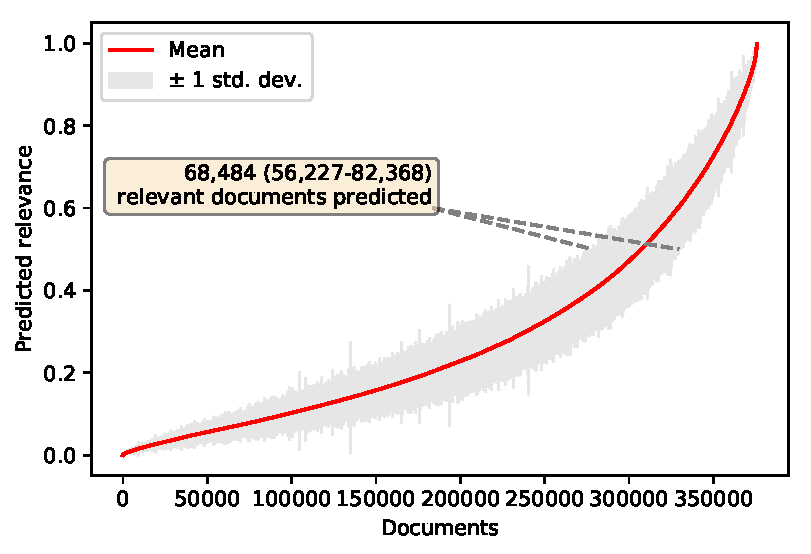
\includegraphics[width=\linewidth]{../plots/prediction_models/predictions_unseen.png}
		\end{figure}
	\end{column}
	\begin{column}{0.382\linewidth}
		\begin{itemize}
			\item We train 10 classifiers on random partitions of the labelled dataset
			\item This gives us 10 estimates for each unseen document
			\item The mean and standard deviation of these estimates give us an idea, with some uncertainty, of how many documents are in each category
		\end{itemize}
	\end{column}
\end{columns}

\end{frame}

\begin{frame}
\only<1>{
	\begin{figure}
		\includegraphics[width=0.7\linewidth]{../plots/process_diagram/relevant.pdf}
	\end{figure}
}
%\only<2>{
%	\begin{figure}
%		\includegraphics[width=0.7\linewidth]{../plots/process_diagram/relevant_cats.pdf}
%	\end{figure}
%}
\only<2>{
	\begin{figure}
		\includegraphics[width=0.7\linewidth]{../plots/process_diagram/relevant_cats_attrib.pdf}
	\end{figure}
}
\end{frame}

%%%%%%%%%%%%%%%%%%%%%%%%%%%%%%%%%%%%%%%%%%%%%%
%% D&A

\section{Detection and attribution}

\begin{frame}
\tableofcontents[currentsection]
\end{frame}

\begin{frame}{Synthesizing impacts evidence with quantitative detection and attribution evidence}

We know from detection and attribution studies whether observed trends in temperature and precipitation are attributable to human influence on the climate.

\cite{Knutson2013, Knutson2018} show this on a grid cell level

\begin{columns}
	\begin{column}{0.65\linewidth}
		\includegraphics[width=\linewidth]{images/knutson_precip_da}
	\end{column}
	\begin{column}{0.35\linewidth}
		\includegraphics[width=\linewidth]{images/knutson_temp_da}
	\end{column}
\end{columns}

We can combine this with information from our database of impacts evidence, in which the locations, and the climate drivers have been predicted

\end{frame}

\begin{frame}{Synthesising impacts with D\&A evidence}
\begin{columns}
	\begin{column}{0.4\linewidth}
		\includegraphics[width=\linewidth]{../plots/maps/sudan_precipitation.png}
	\end{column}

	\begin{column}{0.4\linewidth}
		\includegraphics[width=\linewidth]{../plots/maps/sudan_gridcell_count.png}
	\end{column}
\end{columns}

\begin{itemize}
	\item 11 out of 27 gridcells in Sudan contain a reduction in rainfall attributable to human influence on the climate
	\item Each study referring to Sudan (as the smallest identifiable geographical entity)  and predicted to document impacts driven by precipitation refers to a place where around 41\% of the gridcells are known to have anthropogenic changes in precipitation
\end{itemize}
\end{frame}

\begin{frame}{Synthesising impacts with D\&A evidence}
\begin{columns}
\begin{column}{0.4\linewidth}
	\includegraphics[width=\linewidth]{../plots/maps/sudan_precipitation_studies.png}
\end{column}

\begin{column}{0.4\linewidth}
	\includegraphics[width=\linewidth]{../plots/maps/sudan_precipitation_study_places.png}
\end{column}
\end{columns}

\begin{itemize}
\item 7 studies refer to Sudan (as the smallest identifiable geographical entity), and Sudan has 27 gridcells
\item We apportion these studies to the relevant gridcells, calculating that each gridcell in Sudan has $\frac{7}{27}$ studies referring to it
\item We do the same for each further geographical entity
\end{itemize}
\end{frame}

\begin{frame}{We can show the amount of each type of study in each region}

\begin{columns}
	\begin{column}{0.7\linewidth}
		\begin{figure}
			\includegraphics[width=\linewidth]{../plots/maps/study_type_continent.png}
		\end{figure}
	\end{column}
	\begin{column}{0.3\linewidth}
		 \small
		\begin{itemize}
			\item In North America, most studies refer to places and drivers where a minority of gridcells show an attributable trend
			\item In Africa, the opposite is the case
		\end{itemize}
	\end{column}
\end{columns}

\end{frame}

\begin{frame}{The combination of evidence types at a grid cell level shows where we have lots or little evidence of each type}

\begin{figure}
	\includegraphics[width=\linewidth]{../plots/maps/gridcells_da_studies_temp_2_5_global.png}
\end{figure}

\end{frame}

\begin{frame}{In Europe, we know a larger amount about sectoral impacts in areas we know are warming due to human influence on the climate than in Africa}

\begin{columns}
	\begin{column}{0.6\linewidth}
		\begin{figure}
			\includegraphics[width=\linewidth]{../plots/maps/gridcells_da_studies_temp_2_5_Europe.png}
		\end{figure}
	\end{column}
	\begin{column}{0.4\linewidth}
		\begin{figure}
			\includegraphics[width=\linewidth]{../plots/maps/gridcells_da_studies_temp_2_5_Africa.png}
		\end{figure}
	\end{column}
\end{columns}

Further, impact studies on the effects of human-induced warming in Africa are concentrated in South Africa and East Africa

\end{frame}


\begin{frame}{We are less certain about human influence on precipitation trends, but in China, India, Europe, Southern and Eastern Africa, and the US, the impacts of precipitation trends are frequently studied }

\begin{figure}
	\includegraphics[width=\linewidth]{../plots/maps/gridcells_da_studies_precip_2_5_global.png}
\end{figure}

\end{frame}

\begin{frame}{There are large parts of Africa we know are getting drier because of climate change, but we know little about the effects.}

\begin{columns}
	\begin{column}{0.6\linewidth}
		\begin{figure}
			\includegraphics[width=\linewidth]{../plots/maps/gridcells_da_studies_precip_2_5_Europe.png}
		\end{figure}
	\end{column}
	\begin{column}{0.4\linewidth}
		\begin{figure}
			\includegraphics[width=\linewidth]{../plots/maps/gridcells_da_studies_precip_2_5_Africa.png}
		\end{figure}
	\end{column}
\end{columns}

In Europe, the effects of precipitation change are more frequently studied, even where we cannot attribute changes to human influence.

\end{frame}


%%%%%%%%%%%%%%%%%%%%%%%%%%%%%%%%%%%%%%%%%%%%%%
%% Conclusions
\section{Conclusions}

\begin{frame}
\tableofcontents[currentsection]
\end{frame}

\begin{frame}{A growing body of literature on impacts}

\begin{columns}
	\begin{column}{0.382\linewidth}
		\includegraphics[width=\linewidth]{../plots/literature_distribution/PY_continent_n.pdf}
		
		\includegraphics[width=\linewidth]{../plots/literature_distribution/PY_continent_shares.pdf}
	\end{column}
	\begin{column}{0.618\linewidth}
		\begin{itemize}
			\item There are now hundreds of impacts studies published every year about every continent
			\item There has been huge growth in Asia over the last decade			
		\end{itemize}
	
	\medskip Note that these are rough numbers, for about 27\% of studies, no place could be found with confidence. A further 9\% of studies referred to non-national or supranational geographical entities which could not be easily assigned to a continent.
	\end{column}
\end{columns}

\end{frame}

%\begin{frame}{}
%
%\begin{columns}
%	\begin{column}{0.382\linewidth}
%		\begin{itemize}
%			\item<1-> Lots of the new studies on Asia have been about Detection (is there a regional climate trend)
%			\item<2-> There is also more literature on human impacts and the water cycle in Asia
%			\item<3-> On human impacts, Africa is as much studied as anywhere apart from Asia
%			
%		\end{itemize}
%	\end{column}
%	\begin{column}{0.618\linewidth}
%		\only<1->{\includegraphics[width=\linewidth]{../plots/literature_distribution/PY_continent_attrib.pdf}}
%		\only<2->{\includegraphics[width=\linewidth]{../plots/literature_distribution/PY_continent_impact.pdf}}
%		
%	\end{column}
%\end{columns}
%
%\end{frame}

\begin{frame}{Conclusions}

\begin{itemize}
	\item We identify a large body of evidence about climate impacts, including 17,273 studies documenting impacts in areas where we know at least a part of which are changing due to human influence on the climate (11,089 studies where the majority of gridcells show attributable trends)
	\item What we know about the effects of a changing climate on human and natural systems does not always match with what we know about how (and where) humans are driving changes in climate variables 
\end{itemize}

\textbf{But}, 

\begin{itemize}
	\item Current results only show studies in Web of Science, so definitely do not show all relevant studies
	\item Although our query returned all papers in the relevant AR5 section, it may still miss potentially relevant literature.
	\item Study identification is approximate and uncertain
	\item Geoparsing is also inexact, and is unable to grasp fuzzy geographical content e.g. "Western China"
	\item In large parts of the world, we do not even know reliably if precipitation and temperature are changing
\end{itemize}

\end{frame}

\begin{frame}{Outlook - an interactive atlas of climate impacts evidence}

What can show here are static headline results. What would be most useful for assessment-makers is an interactive platform where evidence can be searched for by sector, type and location. We plan to create such a platform to accompany the paper. 

\medskip

Additionally, we are in the process of incorporating literature from Scopus and MEDLINE, and potentially lens.org.
\end{frame}



\begin{frame}{Summary - Scaling up assessments of regional impacts of climate change: a rapid, computer-assisted systematic map}

\begin{columns}
	\small
	\begin{column}{0.5\linewidth}
		\begin{itemize}
			\item In a large collaborative coding exercise, we examined thousands of papers \textit{potentially} relevant to understanding observed impacts of climate change
			\item We used machine learning to identify tens of thousands of studies \textit{likely} to be relevant.
			\item We predicted the sector, climate driver, evidence type and location for each of these studies
			\item We used the location and predicted climate driver to synthesise this information with existing quantitative Detection and Attribution knowledge.
		\end{itemize}
	\end{column}

	\begin{column}{0.5\linewidth}
		
		\begin{block}{Takeaways}
			\begin{itemize}
				\item Machine learning can inform and support global environmental assessments
				\item We have lots of evidence of observed impacts of climate change, including 17,000 studies documenting impacts in areas we know are changing due to human influence on the climate
				\item What we know about the effects of a changing climate on human and natural systems does not always match with what we know about how (and where) humans are driving changes in climate variables 
			\end{itemize}
		\end{block}
		
	\end{column}
\end{columns}



\begin{center}
	\line(1,0){250}
	
	\medskip
	
	\textbf{Thanks!}
	
	\medskip
	
	Contact: \url{callaghan@mcc-berlin.net}

\end{center}



\end{frame}

%%%%%%%%%%%%
%% Bib
\begin{frame}{Bibliography}
\bibliography{../mendeley}
\end{frame}

\end{document}